% !TeX root = ../thuthesis-example.tex

\chapter{随机块模型的精确恢复问题}


\section{基于玻茨模型的算法}
类似于\ref{sec:sibm_model}节
介绍的SIBM模型,我们将
随机块模型
与 \ref{sec:ising} 节介绍的 玻茨模型
复合起来可得到随机块-玻茨模型。该模型可以看成是SIBM模型的推广,
每个节点由两状态变成了多状态。由于我们的研究重点并非
从随机块-玻茨模型的多个样本恢复节点的原始标签,而是利用
玻茨模型对随机块模型进行社群发现,因此我们首先给出
由随机块模型生成的图上定义的玻茨模型:
\begin{definition}\label{def:ising}
	给定从$\SSBM(n,k,\A,\B)$ 中生成的随机图 $G$,
    定义在$G$上的玻茨模型($k$个状态的伊辛模型)带有两个参数 $\gamma,\beta>0$,
	并且是关于状态向量$\sigma\in W^n$ 的概率分布
。该分布的概率质量函数为
\begin{align} \label{eq:isingma}
	P_{\sigma|G}(\sigma=\bar{\sigma})=\frac{\exp(-\beta H(\bar{\sigma}))}{Z_G(\gamma,\beta)}
	\end{align}
其中能量函数$H(\bar{\sigma})$的定义是
\begin{equation}\label{eq:energy}
	H(\bar{\sigma}) := \gamma \frac{\log n}{n} \sum_{\{i,j\}\not\in E(G)} \delta(\bar{\sigma}_i, \bar{\sigma}_j)
	- \sum_{\{i,j\}\in E(G)} \delta(\bar{\sigma}_i, \bar{\sigma}_j)
	\end{equation}
	
	$P_{\sigma|G}$ 中的下标表示该分布依赖于$G$,
    $Z_G(\gamma,\beta)$ 是该分布的归一化常数。
\end{definition}

式\eqref{eq:isingma}中
各符号的含义同式\eqref{eq:canonical_ensemble}。
而表示汉密尔顿能量的式\eqref{eq:energy}
则是式\eqref{eq:ising_modified}的推广。
当  $k=2$ 时 式 \eqref{eq:energy}
在评注\ref{rem:equivalence_H_energy}的意义下
退化成 式 \eqref{eq:ising_modified}。 

这里的能量函数$H(\bar{\sigma})$ 同样有两部分组成:
没有边相连的节点之间排斥力的势能和
有边相连的节点之间吸引力的势能。
$\gamma$ 参数衡量了两种势能之间的比率而
$\frac{\log n}{n}$ 则是对由于边的数量不均匀造成两种势能量阶不同的修正项,
因为两节点间有边相连的概率仅为 $O(\frac{\log n}{n})$。

定义 \ref{def:ising} 实际上给出了一个估计$X$的随机算法 $\hat{X}^*$。
这里,$\hat{X}^*$ 表示产生于玻茨模型的一个样本,
记作$\hat{X}^* \sim \textrm{Potts}_G(\gamma, \beta)$。
沿用评注\ref{rem:metric_exact_recovery} 中的记号,
使用$\hat{X}^*$估计$X$在精确恢复度量下的错误概率
记为 $P_e(\hat{X}^*) := \sum_{G \in \cG_n} P_G(G) P_{\sigma | G}(S^c_k(X))$。
类似定理\ref{thm:sibm_phase_trans}中关于 SIBM 模型的讨论,
玻茨模型的两个参数$(\gamma, \beta)$ 的取值
对$P_e(\hat{X}^*)$
也有着决定性的作用。
当它们取合适的值时, 
$ P_e(\hat{X}^*)\to 0$,
随机块模型的精确恢复可以实现。
反之,如果 $(\gamma, \beta)$ 取其他值时,
$P_e(\hat{X}^*) \to 1$。
这两种情况可总结为如下的定理:

\begin{theorem}\label{thm:phase_transition}
	假设 $\sqrt{a} - \sqrt{b} > \sqrt{k}$,
	定义函数 $g(\beta)$ 和 $ \tilde{g}(\beta)$ 如下:
	\begin{equation}
		\label{eq:g_beta_main_article}
		g(\beta) = \frac{be^{\beta} + a e^{-\beta}}{k} - \frac{a+b}{k} +1
	\end{equation}
	且
	\begin{equation}
		\label{eq:g_tilde_beta_main_article}
	\tilde{g}(\beta) = \begin{cases}
	g(\beta) & \beta \leq \bar{\beta} = \frac{1}{2}\log \frac{a}{b} \\
	g(\bar{\beta}) = 1 - \frac{(\sqrt{a} - \sqrt{b})^2}{k} & \beta > \bar{\beta}
	\end{cases}
	\end{equation}
	其中
	$\bar{\beta} =  \displaystyle\arg\min_{\beta > 0} g(\beta)$。
	令 $\beta^*$ 定义成
	\begin{equation}\label{eq:beta_star}
	\beta^* = \log\left(\frac{a + b - k - \sqrt{(a + b - k)^2 - 4 a b)}}{2  b}\right)
	\end{equation}
	可以验证 $\beta^*$ 是方程 $g(\beta) = 0$ 的解 并且满足  $\beta^* < \bar{\beta}$。
	则取决于 $(\gamma, \beta)$ 如何取值,对于给定的 $\epsilon > 0$, 
	$G\sim \SSBM(n, k, \A, \B)$, $\hat{X}^* \sim \textrm{Potts}_G(\gamma, \beta)$,
	当 $n$ 充分大时, 我们有:
	\begin{enumerate}
	\item 当 $\gamma > b$ 且 $\beta > \beta^*$ 时,$P_e(\hat{X}^*) \leq n^{\tilde{g}(\beta)/2 + \epsilon}$;
	\item 当 $\gamma > b$ 且 $\beta < \beta^*$ 时,$P_a(\hat{X}^*) \leq (1+o(1))\max\{n^{g(\bar{\beta})}, n^{-g(\beta) + \epsilon}\}$;
	\item 当 $\gamma < b$ 时,对于任意给定的 $C>0$	均有 $P_a(\hat{X}^*) \leq \exp(-C n)$。
	\end{enumerate}
\end{theorem}

\begin{figure}[H]
	\begin{subfigure}{0.43\textwidth}
		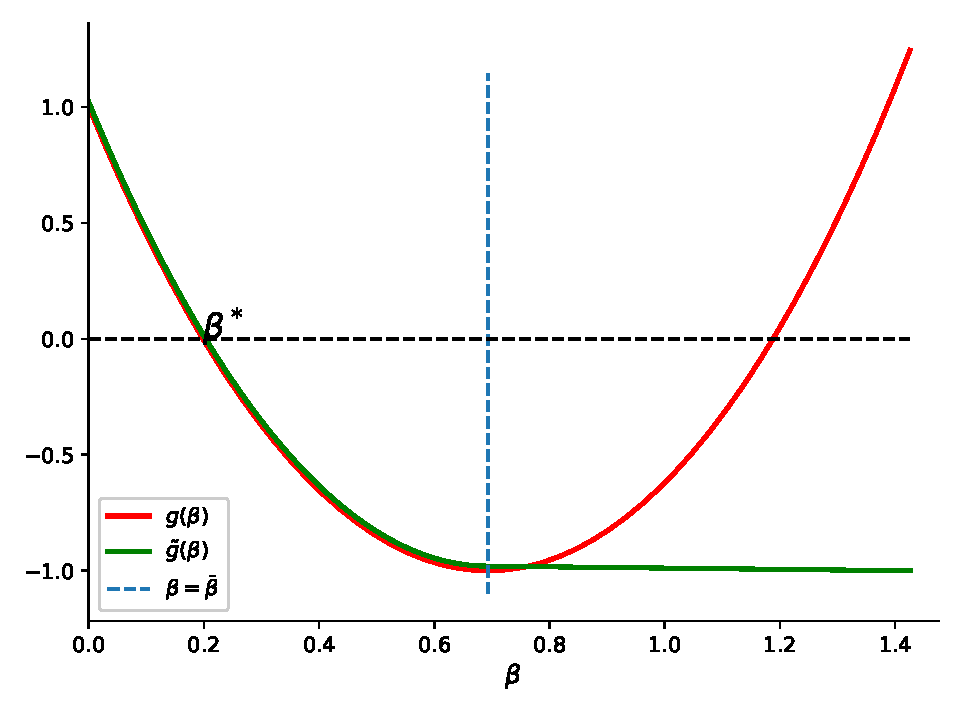
\includegraphics[width=\textwidth]{g-16-4-2.pdf}
		\caption{当 $a=16,b=4,k=2$时,$g(\beta)$和
		$\tilde{g}(\beta)$的函数图像}\label{fig:g}
	\end{subfigure}~
	\begin{subfigure}{0.55\textwidth}
		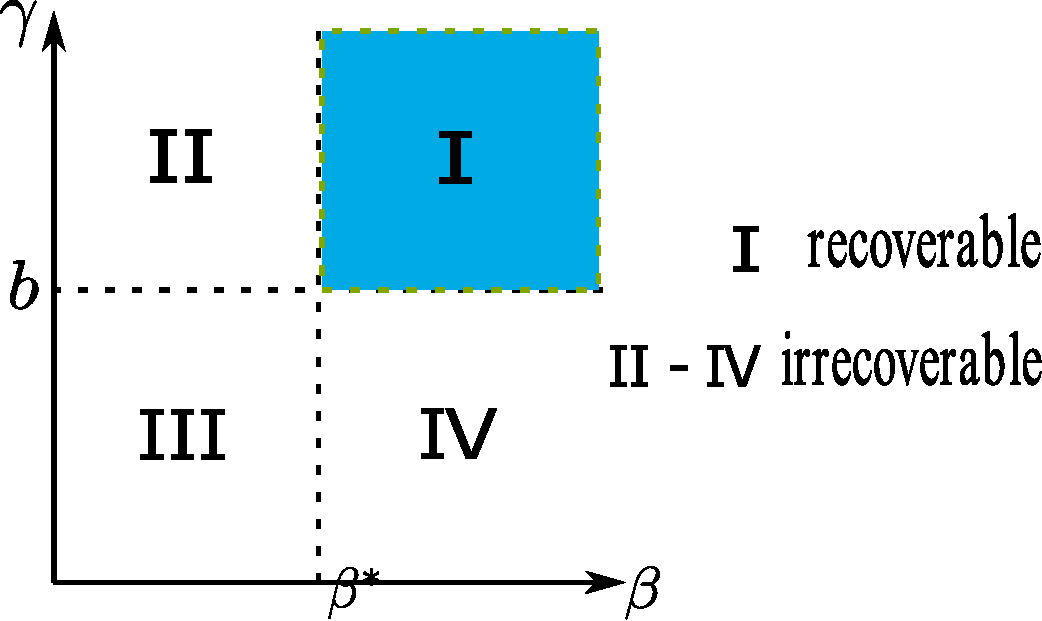
\includegraphics[width=\textwidth]{phase_trans.pdf}
		\caption{
			在 $(\beta, \gamma)$ 平面内
			相变区域图示。
			随机块模型的精确
			恢复仅在区域 I 可实现。}\label{fig:pt}
	\end{subfigure}
	\caption{定理 \ref{thm:phase_transition}
	的图示}
	\label{fig:phase_transition_theorem_illustration}
\end{figure}

与式\eqref{eq:beta_star_sibm}的情形类似,注意到条件$\sqrt{a} - \sqrt{b} > \sqrt{k}$保证了
式\eqref{eq:beta_star}中的根号下的项非负。
这个条件来自于定理\ref{thm:sbmk_phase_transition},
保证了随机块模型本身精确恢复可实现。


通过简单的计算可知,对于 $\beta> \beta^*$ 我们有
$\tilde{g}(\beta) < 0$ 而 对于 $\beta < \beta^*$有
$g(\beta)>0$。
另外,由 $\sqrt{a} - \sqrt{b} > \sqrt{k}$ 可知
$g(\bar{\beta}) < 0$。
$g(\beta), \tilde{g}(\beta)$ 的图像
如图 \ref{fig:phase_transition_theorem_illustration}a 所示。
因此, 对于充分小的
$\epsilon$ 并且当 $n \to \infty$,
定理\ref{thm:phase_transition} 中给出的上界
均至少以多项式的速度趋向于 $0$。
从而定理\ref{thm:phase_transition} 
刻划了
玻茨模型的相变性质。
如图\ref{fig:phase_transition_theorem_illustration}b所示
, 对于玻茨模型, 只有参数$(\beta, b)$落在区域I时,
随机块模型的精确
恢复才能实现。

定理\ref{thm:phase_transition}
也可以从$\sigma$的边缘分布的角度理解。
玻茨模型取到某个特定状态$\bar{\sigma}$的概率为
 $\sigma: P_{\sigma}(\sigma =\bar{\sigma})
=\sum_{G \in \cG_n}P_G(G)P_{\sigma |G}(\sigma=\bar{\sigma})$.
我们用符号 $D(\sigma, \sigma')$
表示
$\sigma$ 相比于它的所有置换其本身离 $\sigma'$ 最近
这个事件。
也即
\begin{equation}
	\label{eq:D_sigma_sigma_prime}
D(\sigma, \sigma') := \{ \sigma = \arg\min_{f \in S_k} \Dist(f(\sigma), \sigma')  \}
\end{equation}

则 定理 \ref{thm:phase_transition} 
对边缘分布 $P_{\sigma}$ 蕴含着如下的论断
:
\begin{corollary}\label{cor:phase4}
假设 $\gamma > b$, 取决于 $\beta$ 的取值我们有
\begin{enumerate}
	\item 当 $\beta > \beta^*$时,$P_{\sigma}(\sigma = X | D(\sigma, X))  = 1-o(1)$;
	\item 当 $\beta < \beta^*$时,$P_{\sigma}(\sigma = X | D(\sigma, X))  = o(1)$。
\end{enumerate}
\end{corollary}

下面我们简单阐述下 定理 \ref{thm:phase_transition} 证明的思路。
该思路主要通过对翻转一个状态的前后能量差的分析来估计概率的主项。
下面的引理总结了翻转一个状态汉密尔顿能量的变化:
\begin{lemma}\label{lem:lemmaDiff}
	假设 $\bar{\sigma}'$ 仅在第$r$个位置上与 $\bar{\sigma}$ 不同,
	差别为 $\bar{\sigma}'_r = \omega^s \cdot \bar{\sigma}_r$。
	则 $\bar{\sigma}'$ 和 $\bar{\sigma}$ 的能量差为
\begin{align}
	H(\bar{\sigma}') - H(\bar{\sigma}) &= (1+\gamma \frac{\log n}{n})\sum_{i \in N_r(G)} J_s(\bar{\sigma}_r, \bar{\sigma}_i)
	\notag \\
	&+ \gamma \frac{\log n}{n} (m(\omega^s \cdot \bar{\sigma}_r)-m(\bar{\sigma}_r)+1) \label{eq:DeltaH}
	\end{align}
	上式中 $m(\omega^j) := |\{i \in [n] | \bar{\sigma}_i = \omega^j | \}$, $N_r(G):=\{j | (r, j) \in E(G) \}$ 且 $J_s(x, y) = \delta(x, y) - \delta(\omega_s \cdot x, y)$.
\end{lemma}
引理 \ref{lem:lemmaDiff} 提供了用以比较两个相邻状态的    概率
的方法,即:
\begin{equation}\label{eq:Pratio}
\frac{P_{\sigma |G } (\sigma = \bar{\sigma}')}{P_{\sigma |G } (\sigma = \bar{\sigma})}
= \exp(-\beta(H(\bar{\sigma}') - H(\bar{\sigma})))
\end{equation}

另外, 我们注意到 因为图的边的数量是稀疏的,每个节点
平均有 $O(\log n)$ 个相连的邻居节点。
按照式 \eqref{eq:DeltaH} 
计算能量差的时间复杂度也是 $O(\log n)$。

当 $H(\bar{\sigma}') > H(\bar{\sigma})$ 时, 
由式\eqref{eq:Pratio} 可得
$P_{\sigma | G}(\sigma = \bar{\sigma}')$
小于
$P_{\sigma | G}(\sigma = \bar{\sigma})$。
粗略而言, 如果
$ \sum_{\Dist(\sigma', X)=1}\exp(-\beta(H(\bar{\sigma}') - H(X))) $
收敛到零,
我们可以预期,与$S_k(X)$不同的所有其他状态的概率收敛到零。
与之相反, 如果
$ \sum_{\Dist(\sigma', X)=1}\exp(-\beta(H(\bar{\sigma}') - H(X))) $
趋于无穷大,
则 $P_{\sigma}(S_k(X))$ 趋于零。
此种分析展示了证明定理 \ref{thm:phase_transition}的
主要思路。
严格的证明参见附录 \ref{sec:appendix_theorem_proof_phase_trans}。

\section{参数估计}

\section{与其他算法的联系}

在附录中,我们给出一个这个论断的数学推导。